



Basierend auf Azure AI Cognitive Service ist AI Builder ein Tool, welches zum Erstellen und Trainieren von Modellen, ohne das Schreiben von Code dient. Die Integration mit Power Apps und Power Automate ist eine Funktion, die den Nutzern die Möglichkeit bietet, bestehende Geschäftsanwendungen zu erweitern, und zu verbessern.
Microsoft Power Plattform ist eine Low-Code-Plattform, die es Unternehmen bewilligt, Geschäftsprozesse zu automatisieren. Power Plattform umfasst drei Hauptprodukte: Power BI, PowerApps und Flow.
Mit dem AI Builder ist es möglich, auf einfache Weise Prozesse zu automatisieren und Ergebnisse vorherzusagen. AI Builder ist eine schlüsselfertige Lösung, die die Leistungsfähigkeit der künstlichen Intelligenz von Microsoft mit wenigen Mausklicks anwendbar macht. Mit dem AI Builder kann man Anwendungen Intelligenz beifügen, auch wenn Sie keine Programmier- oder Data-Science-Kenntnisse haben.

\subsection{Benutzerdefinierte Modelle}

Der erste Schritt bei der Erstellung eines KI-Modells besteht darin, festzustellen, ob für den Anwendungsfall bereits vorgefertigte oder bereits trainierte Modell vorhanden sind. Ist dies nicht der Fall, stehen in der Benutzeroberfläche des AI Builders fünf Modelle zur Verfügung:

\begin{enumerate}
    \item Category Classification
    \item Entity Extraction
    \item Form Processing
    \item Object Detection
    \item Prediction
\end{enumerate}

\begin{figure}[h]
    \centering
    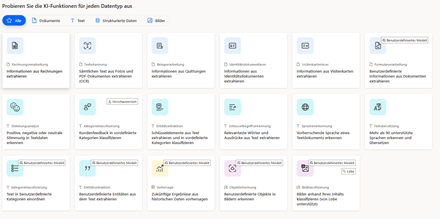
\includegraphics[scale=0.9]{sections/cloud-computing/images/ai-builder-models.png}
    \caption{AI-Builder Modelle}
    \label{fig:kimldl-comparison}
\end{figure}

\subsubsection{Category Classification}

Bei diesem Ansatz wird ein Modell verwendet beziehungsweise trainiert, um große Mengen an Textdaten, Dokumenten oder sonstige Textdatenquellen zu analysieren, und den Text zu klassifizieren. Besonders hilfreich ist dieses Modell, um Spam zu identifizieren, und entsprechend zu behandeln. Zuerst muss das Modell mit Trainingsdaten trainiert werden. Das Zeichenlimit für jede Textprobe liegt bei fünftausend Zeichen.

Die Analysen, die dieses Modell liefert, können auch als Input für andere KI-Lösungen verwendet werden. Wichtig hierbei ist, dass für jeden Tag mindestens zehn Textproben bereitgestellt werden, ansonsten sinkt die Wahrscheinlichkeit ein genaues Ergebnis zu erzielen.

\subsubsection{Entity Extraction}

Hier werden wichtige Textelemente identifiziert, ferner den definierten Kategorien zugeordnet. Die Ergebnisse werden dabei, entsprechend den Anforderungen, standardisiert und strukturiert. Auch hier werden wieder mindestens 10 Datensätze benötigt, um mit dem Trainieren des Modells beginnen zu können. Das Modell ist anpassbar, indem man neue Entitätstypen mit wenigen Trainingsdaten erstellt oder bestehende Entitätstypen modifiziert. Der Ai Builder verfügt über vorgefertigte Trainingsdaten, die zur Erweiterung der eigenen Trainingsdaten verwendet werden können.

\subsubsection{Form Processing}

Die Formularverarbeitung ist das KI-Modell, das Daten aus Formularen, auch aus Papier- oder PDF-Dokumenten, extrahiert. Es werden fünf Beispielformluare benötigt, ums es zu trainieren, die Felder eines Dokuments zuzuordnen und eine funktionierende Anwendung zu erstellen. Diese Lösung wird verwendet um Rechnungen und Aufträge zu erfassen. Beispielsweise ist es möglich, das Modell zu trainieren und einen Ablauf zu erstellen, der automatisch Schlüsselinformationen aus Bestelldokumenten erkennt, extrahiert und anschließend eine E-Mail an den zuständigen Mitarbeiter sendet.

Die empfohlenen Formate für die Eingabedaten sind .jpg, .png und .pdf. Die Gesamtgröße der, für das Training verwendeten, Dokumente, darf insgesamt 50 MB nicht überschreiten.

\subsubsection{Object Detection}

Die Objekterkennung wird verwendet, um Objekte auf Fotos oder Videos zu erkennen. Dieses Modell kann verwendet werden, um bestimmte Informationen von Produkten oder Maschinen zu erhalten. Ebenfalls hilfreich kann dieses Modell bei mobilen Anwendungen sein.

Für das Training werden mindestens 15 Fotos von jedem Objekt benötigt; je mehr Fotos, desto genauer ist das Modell.  Um eine korrekte Identifiezierung zu gewährleisten, sollten die Fotos möglichst verschiedene Hintergründen beinhalten. Ebenfalls empfehlenswert ist es, Fotos von Objekten aus diversen Entfernungen und Winkeln bereitzustellen. Es ist zu beachten, dass die Trainingsbilder im .jpg-, .bmp- oder png-Format vorliegen müssen und insgesamt 6 MB pro Training nicht überschreiten dürfen. Die Grenze von 256 x 256 Pixel soll jedoch nicht unterschritten werden.

\subsubsection{Prediction} 

Bei diesem Modell werden große Mengen an alten Daten analysiert, um darin Muster zu erkennen. Das gewonnene Wissen wird dann verwendet, um diese Muster in neuen Datensätzen zu erkennen, und Vorhersagen zu treffen.

Zum Trainieren des Modells werden mindestens 10 Zeilen mit historischen Werten, für jede Klasse der Datenspalte "Label", benötigt. Die Mindestanzahl der Zeilen für das Training liegt bei 50, aber ein Minimum von 1.000 Zeilen gewährleistet die erfolgreichsten Ergebnisse.

\subsection{AI-Builder in der Praxis}

Um den AI-Builder für den gewünschten Use-Case am effektivsten zu nutzen, hat sich das Diplomarbeitsteam dazu entschieden, das Modell des Form Processing zu verwenden. Der gewünschte Use-Case ist mehrere, im Vorhinein definierte Felder aus einer Eingangsrechnung, im PDF, zu extrahieren und anschließend zu markieren. 
Die untenstehende Abbildung dient zur veranschaulichung einer solchen Eingangsrechnung (Siehe Abbildung \ref{fig:example-invoice-figure}). Folgende Schritte sind ein wesentlicher Bestandteil, um ein Modell zu erstellen, dass auf spezielle Eingangsrechnungen trainiert ist:

\begin{enumerate}
    \item Zu extrahierende Felder definieren
    \item Trainingsdaten bereitstellen
    \item Trainingsdaten mit Tags versehen
    \item Modell trainieren und
    \item Modell veröffentlichen
\end{enumerate}

\begin{figure}[h]
    \centering
    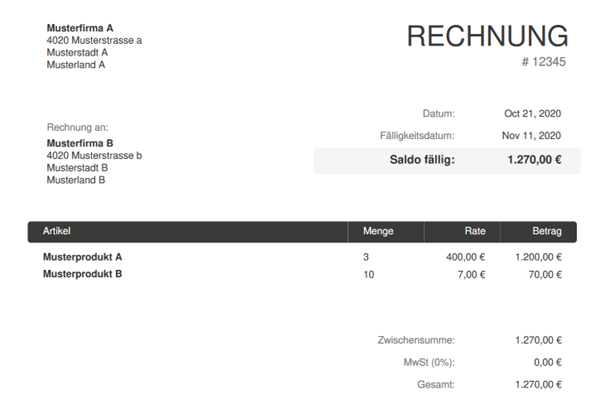
\includegraphics[scale=0.9]{sections/cloud-computing/images/example-invoice.png}
    \caption{Beispiel Eingansrechnung}
    \label{fig:example-invoice-figure}
\end{figure}

Zunächst ist es wichtig zu wissen, welche Felder man aus der ER extrahieren will. In der folgenden Abbildung wird gezeigt, welche Felder bei dieser Arbeit ausgewählt wurden. Jene Felder wurden nur zu Veranschaulichung der Fähigkeiten des AI-Builders ausgewählt:

\begin{figure}[h]
    \centering
    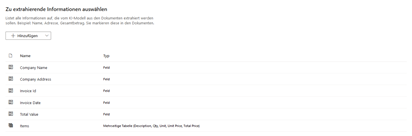
\includegraphics[scale=0.5]{sections/cloud-computing/images/ai-builder-fields.png}
    \caption{AI-Builder Felder}
    \label{fig:ai-builder-fields-figure}
\end{figure}

\begin{enumerate}
    \item Company Name
    \item Company Address
    \item Invoice Id
    \item Invoice Date
    \item Total Value
    \item Items (Mehrseitige Tabelle)
\end{enumerate}

\textbf{Items (Mehrseitige Tabelle)}: Diese Tabelle bietet ein experimentelles Feature, um tabellarische Daten aus einer, in der Rechnung vorhandenen Tabelle zu entnehmen, auch wenn sich die Tabelle über mehrere Seiten zieht. Diese Tabelle enthält wiederrum eigene Daten wie:

\label{enum:InvoiceItemsAttributs}
\begin{enumerate}
    \item Description
    \item Qty (Quantity)
    \item Unit
    \item Unit Price
    \item Total Price
\end{enumerate}


Um Daten für das Trainieren des Modells bereitzustellen, ist es notwendig mindestens fünf Beispieldokumente hochzuladen. Nichtsdestotrotz ist für eine hohe Genauigkeit des Modells, sprich wie sicher sich der Algorithmus ist, dass er das richtige Feld markiert hat, von Vorteil mehrere ähnliche Dokumente bereitzustellen. 
Um dem Algorithmus anzutrainieren, welche Felder in dem Dokument vorhanden sind, ist es relevant die Daten in dem Dokument händisch zu markieren, und die zuvor definierten Informationsfelder zu zuweisen. Siehe folgende Abbildung (\ref{fig:ai-builder-tagging-figure})

\begin{figure}[h]
    \centering
    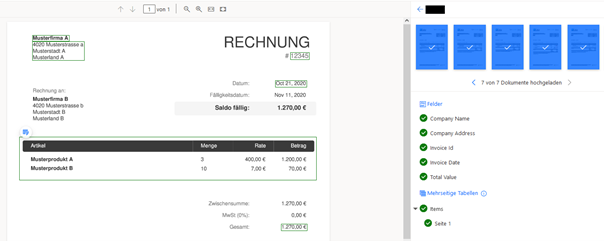
\includegraphics[scale=0.9]{sections/cloud-computing/images/ai-builder-tagging.png}
    \caption{AI-Builder Felder Tagging}
    \label{fig:ai-builder-tagging-figure}
\end{figure}